\documentclass[11pt]{article}

\usepackage{amsmath}
\usepackage{amssymb}
\usepackage[margin=0.68in]{geometry}
\usepackage{booktabs}
\usepackage{enumitem}
\usepackage{fancyhdr}
\usepackage{graphicx}
\usepackage[table]{xcolor}
\usepackage[hidelinks]{hyperref}
\usepackage{listings}
\usepackage{microtype}
\usepackage{tabularx}
\usepackage{tikz}
\usepackage{titlesec}
\usetikzlibrary{arrows.meta,positioning}
\graphicspath{{docs/lessons/assets/}{../assets/}}

\definecolor{Ink}{gray}{0}
\definecolor{CodeGray}{gray}{0.96}
\definecolor{Soft}{gray}{0.90}
\hypersetup
{
    pdftitle={ADK Lesson 023: Inert Load Interlock},
    pdfauthor={Kevin Shanahan},
    pdfsubject={Bounded simulated load intent with distinct request, application, and fault evidence},
    pdflang={en-US}
}
\pagestyle{fancy}
\fancyhf{}
\lhead{\textsc{ADK Lesson 023}}
\rhead{Inert Load Interlock}
\cfoot{\thepage}
\setlength{\headheight}{14pt}
\setlength{\parindent}{0pt}
\setlength{\parskip}{5pt}
\setlist{nosep,leftmargin=1.45em}
\titleformat{\section}{\Large\bfseries\color{Ink}}{\thesection}{0.5em}{}
\titleformat{\subsection}{\large\bfseries\color{Ink}}{\thesubsection}{0.5em}{}
\lstdefinestyle{adkcpp}
{
    language=C++,
    backgroundcolor=\color{CodeGray},
    basicstyle=\ttfamily\small,
    keywordstyle=\color{Ink}\bfseries,
    commentstyle=\color{Ink},
    columns=fullflexible,
    keepspaces=true,
    showstringspaces=false,
    frame=single,
    rulecolor=\color{Ink},
    breaklines=true,
    tabsize=4
}
\newcommand{\checkbox}{\(\square\)}
\newcommand{\blank}[1]{\rule{#1}{0.4pt}}
\newcommand{\lessonbox}[1]{%
  \begin{center}
  \fcolorbox{Ink}{white}{\parbox{0.92\linewidth}{#1}}
  \end{center}}

\begin{document}

\begin{center}
  {\Huge\bfseries Inert Load Interlock}\\[4pt]
  {\Large Requested, applied, and fault are different facts}\\[8pt]
  \textit{Five LEDs make a bounded software policy visible without energizing a load.}
\end{center}

\begin{tabularx}{\linewidth}{@{}>{\bfseries}l X >{\bfseries}l X@{}}
Lesson & 023 --- component & Time & 150--210 minutes\\
Prerequisites & Lessons 001--022 & Board & Arduino Mega 2560\\
Primary evidence & D13, D38, D40, D41, D12 & Status & physical acceptance open\\
Energy class & E1: USB and resistor-limited LEDs only\\
\end{tabularx}

\lessonbox{\textbf{Hard boundary.} Fan, pump, and heater are names for three
LED channels. Do not connect a relay, motor, pump, heater, transistor board,
external load supply, or mains circuit. Command admission is a software fact,
not power evidence. ADK is not a functional safety controller.}

\section{Mission}

Build an observable chain with no energetic load:
\[
\text{request}\rightarrow\text{admission policy}\rightarrow
\text{one applied intent}\rightarrow\text{LED evidence}.
\]
At the end you should be able to explain why these statements differ:

\begin{enumerate}
  \item a channel was requested;
  \item policy admitted one active intent;
  \item an indicator was commanded;
  \item the indicator visibly responded; and
  \item a real load received power.
\end{enumerate}

This lesson can establish the first four only. The fifth is deliberately
outside the circuit.

\section{Orientation and wiring}

\begin{center}
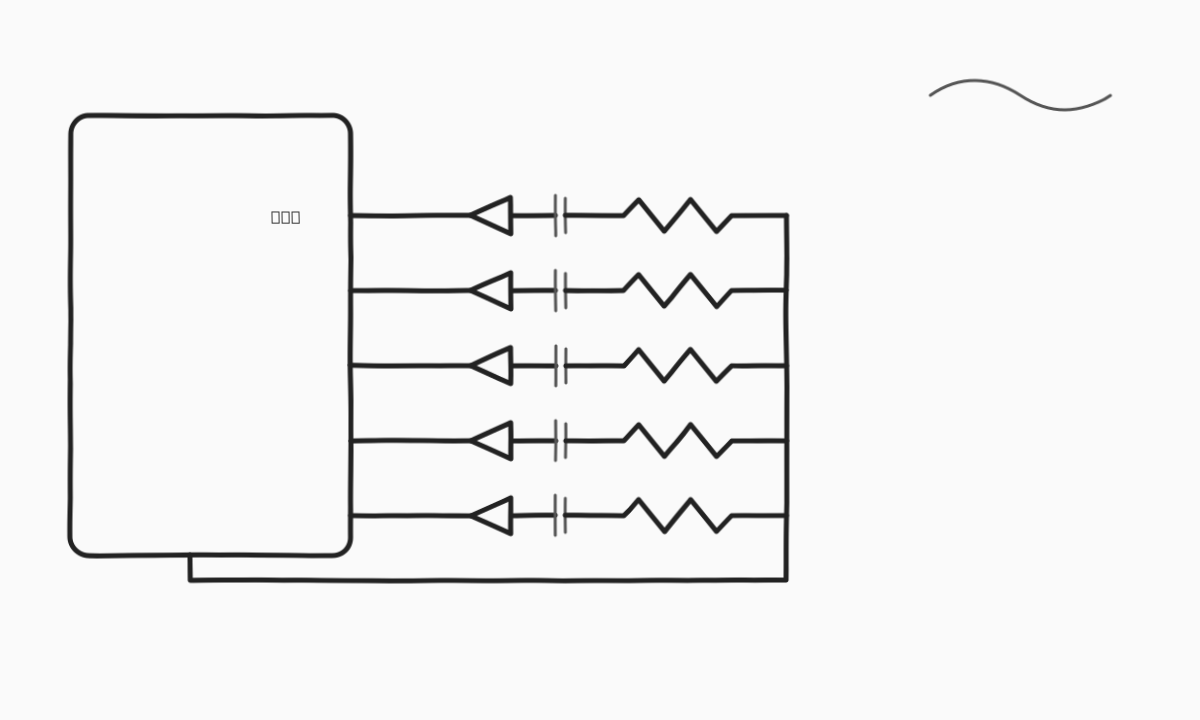
\includegraphics[width=0.94\linewidth]{023-inert-load-pencil.png}
\end{center}
\textit{Alternative text: a pencil-style Mega 2560 orientation drawing. D13
shows a request pulse; D40, D38, and D41 show applied fan, pump, and heater
intent; D12 shows a latched fault. Each external LED returns through its own
resistor to the common ground. No load or relay is connected.}

\begin{tabularx}{\linewidth}{@{}l l X@{}}
\toprule
Meaning & Pin & Connection\\
\midrule
Requested intent & D13 & Built-in LED; no external wire\\
Applied pump & D38 & D38 to 220 \(\Omega\), LED anode; cathode to GND\\
Applied fan & D40 & D40 to 220 \(\Omega\), LED anode; cathode to GND\\
Applied heater & D41 & D41 to 220 \(\Omega\), LED anode; cathode to GND\\
Latched fault & D12 & D12 to 1 k\(\Omega\), LED anode; cathode to GND\\
\bottomrule
\end{tabularx}

\textbf{Unpowered inspection.} Remove USB. Confirm LED polarity, one resistor
per LED, a common Mega GND, and no connection to a relay or powered load.
Record resistor measurements: D38 \blank{.55in}, D40 \blank{.55in},
D41 \blank{.55in}, D12 \blank{.55in}.

\section{The object story}

\begin{center}
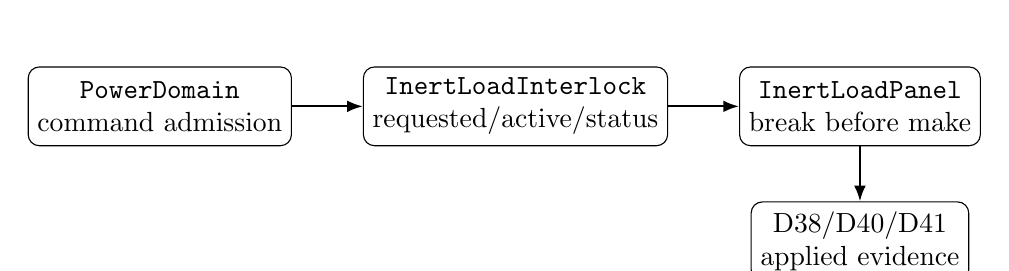
\begin{tikzpicture}[
  node distance=7mm and 9mm,
  box/.style={draw,rounded corners,align=center,minimum height=10mm},
  arrow/.style={-{Latex[length=2mm]},thick}
]
  \node[box] (gate) {\texttt{PowerDomain}\\command admission};
  \node[box,right=of gate] (policy) {\texttt{InertLoadInterlock}\\requested/active/status};
  \node[box,right=of policy] (panel) {\texttt{InertLoadPanel}\\break before make};
  \node[box,below=of panel] (leds) {D38/D40/D41\\applied evidence};
  \draw[arrow] (gate) -- (policy);
  \draw[arrow] (policy) -- (panel);
  \draw[arrow] (panel) -- (leds);
\end{tikzpicture}
\end{center}

\texttt{InertLoadInterlock} owns no pin. It records one requested selection
and at most one active intent. Each \texttt{IndicatorPump} owns one indicator
endpoint. \texttt{InertLoadPanel} borrows the three outputs in fan, pump,
heater order and renders the applied selection; it cannot outlive them. These
relationships are not evidence that a real load is safe.

\subsection{Lifecycle}

Construction is inert. Initialization establishes \texttt{None}. Repeated
initialization is idempotent. Shutdown selects all-off and releases owned
endpoints. Destruction calls shutdown and remains safe during caller exception
unwinding, although ADK itself does not throw.

A revoked admission causes \texttt{HardwareFailure}, clears active intent, and
leaves the failure sticky. Restoring admission does not silently retry.
Recovery is explicit: shutdown, correct the external condition, initialize,
then issue a new request.

\subsection{One bounded status value}

\begin{lstlisting}[style=adkcpp]
const adk::Status status = interlock.select (requestedLoad);

if (!status.ok ())
{
    observeFailure (status);
}
\end{lstlisting}

Pass the complete value to the observation boundary. Use \texttt{error()} only
when policy needs the underlying code. \texttt{transient()} classifies a cause;
it never authorizes an unbounded retry.

\section{Read the snapshot}

\begin{tabularx}{\linewidth}{@{}l l l X@{}}
\toprule
Requested & Active & Status & Meaning\\
\midrule
Pump & Pump & Ok & Pump indicator intent was admitted\\
Heater & Heater & Ok & Prior channel cleared before heater applied\\
None & None & Ok & Deliberately inactive\\
Pump & None & HardwareFailure & Request recorded; admission failed closed\\
Invalid value & unchanged & InvalidArgument & Prior valid state preserved\\
\bottomrule
\end{tabularx}

The request pulse on D13 establishes that a selection attempt occurred.
Exactly one of D38, D40, and D41 renders \texttt{active}. D12 renders a
reported fault. Do not collapse those observations into a single ``working''
light.

\section{Experiment A: mutual exclusion}

\textbf{Predict.} Write the expected applied LED after each request.

\begin{tabularx}{\linewidth}{@{}c l l l X@{}}
\toprule
Step & Request & D13 & Applied LED & Prediction\\
\midrule
1 & Fan & pulse & D40 & \blank{1.3in}\\
2 & Pump & pulse & D38 & \blank{1.3in}\\
3 & Heater & pulse & D41 & \blank{1.3in}\\
4 & None & pulse & none & \blank{1.3in}\\
\bottomrule
\end{tabularx}

\textbf{Observe.} Watch the request pulse before the applied channel changes.
At no instant should two applied indicators remain illuminated.

Record one complete sequence: \blank{3.2in}.

\textbf{Interpret.} Does the sequence support break-before-make? Why?

\blank{4.1in}.

\section{Experiment B: admission fault}

The deterministic host test revokes the borrowed domain while an intent is
active. The Mega teaching sketch may expose the same scenario only through a
fixed, documented simulation; no power path is interrupted.

\begin{enumerate}
  \item Predict the next requested, active, and status fields.
  \item Observe D13, all three applied LEDs, and D12 separately.
  \item Confirm requested may name a load while active remains \texttt{None}.
  \item Restore admission without restarting. Confirm the fault stays sticky.
  \item Restart the lifecycle before making a fresh request.
\end{enumerate}

\begin{tabularx}{\linewidth}{@{}l l l X@{}}
\toprule
Moment & Requested evidence & Applied evidence & Fault evidence\\
\midrule
Before revoke & \blank{.8in} & \blank{.8in} & \blank{.8in}\\
After revoke & \blank{.8in} & \blank{.8in} & \blank{.8in}\\
Admission restored & \blank{.8in} & \blank{.8in} & \blank{.8in}\\
After lifecycle restart & \blank{.8in} & \blank{.8in} & \blank{.8in}\\
\bottomrule
\end{tabularx}

\lessonbox{\textbf{Interpretation limit.} All-off LEDs support fail-closed
software intent. They do not establish galvanic isolation, contact position,
load voltage, or removal of stored energy.}

\section{Fault laboratory}

\begin{tabularx}{\linewidth}{@{}p{0.25\linewidth} X X@{}}
\toprule
Injected condition & Expected public result & Expected evidence\\
\midrule
Selection before initialize & NotInitialized & no applied LED\\
Unknown enum value & InvalidArgument & prior valid selection unchanged\\
Admission revoked & transient HardwareFailure & active all-off; D12 latched\\
Old channel cannot turn off & HardwareFailure & best-effort all-off\\
New channel cannot turn on & HardwareFailure & best-effort all-off\\
Repeated shutdown & Ok cleanup behavior & every applied LED off\\
Destruction while active & no throw, no retained claim & pins released\\
\bottomrule
\end{tabularx}

For each row, distinguish the returned \texttt{Status}, the snapshot, the
recorded endpoint trace, and the physical observation. One cannot substitute
for another.

\section{Shutdown proof}

Resource acquisition and safe electrical state are separate checks.

\begin{enumerate}
  \item \textbf{Acquire:} predict a busy indicator pin causes transactional
        rollback. Host evidence should show every earlier claim released.
  \item \textbf{Inactive:} predict each applied LED is dark before release.
  \item \textbf{High impedance:} with the circuit and meter arranged
        unpowered, observe D38/D40/D41 after shutdown relative to named GND.
  \item \textbf{Reset:} do not infer safe state from a destructor. Remove USB
        power before touching the circuit.
\end{enumerate}

\section{Deterministic proof}

The host suite should exhaust transitions among \texttt{None}, \texttt{Fan},
\texttt{Pump}, and \texttt{Heater}; initialization failures at every endpoint;
old-off and new-on failures; invalid input; asynchronous admission revocation;
sticky faults; explicit recovery; repeated shutdown; and destruction.

The key trace property is:
\[
\forall t,\quad
[\mathrm{fan}(t)]+[\mathrm{pump}(t)]+[\mathrm{heater}(t)]\leq1.
\]
Replay the same admission and request trace twice. Requested, active, status,
and endpoint records must match exactly.

\section{Exercises}

\begin{enumerate}
  \item Draw a state table that distinguishes \texttt{requested} from
        \texttt{active}. Why is one field insufficient?
  \item Explain why \texttt{transient()} must not automatically restart a
        failed selection.
  \item Add a host-only fault at each panel write. Prove the all-off pass is
        attempted without claiming that it succeeds.
  \item Design a two-LED code for requested versus applied without using
        color. State which information is lost.
  \item Explain why a real relay adapter belongs to a different energy class
        and needs independent power-removal evidence.
  \item Explain how \texttt{PanelPumpOutput} borrows
        \texttt{InertLoadPanel}, adapts only its pump channel, and why it must
        not outlive the panel in Lesson 024.
\end{enumerate}

\section{CLI workflow}

\begin{lstlisting}[style=adkcpp]
make host-test
make arduino-Lesson023InertLoadInterlock
make size-Lesson023InertLoadInterlock
make lessons
make lessons-check
make site-check
\end{lstlisting}

Compilation, deterministic replay, and PDF generation are software evidence.
They leave every physical row below open.

\section{Physical acceptance record --- intentionally blank}

\begin{tabularx}{\linewidth}{@{}l X@{}}
\toprule
Field & Record\\
\midrule
Date, person, commit & \\
Mega board/revision & \\
Arduino CLI/core versions & \\
USB supply and measured rail & \\
Instrument and identifier & \\
Measured resistor values & \\
Unpowered wiring inspection & \\
Acquisition prediction/observation & \\
Normal sequence prediction/observation & \\
Mutual-exclusion observation & \\
Fault prediction/observation & \\
Shutdown LED observation & \\
High-impedance observation & \\
Reset and power-removal observation & \\
Deviation and stop condition & \\
\bottomrule
\end{tabularx}

\textbf{Result:} \checkbox\ pass \quad \checkbox\ fail \quad
\checkbox\ not run. Until a named person fills this record from a real bench,
the lesson remains host verified at most.

\section{References and next step}

\begin{itemize}
  \item \href{https://github.com/spincyc/adk/tree/main/examples/Lesson023InertLoadInterlock}
  {Canonical Lesson 023 example}
  \item Interface and tests:
  \url{https://github.com/spincyc/adk/blob/main/src/inert_load_interlock.h}
  and
  \url{https://github.com/spincyc/adk/blob/main/tests/test_inert_load_interlock.cpp}
  \item ATmega2560:
  \url{https://www.microchip.com/en-us/product/atmega2560}
  \item ADK safety model:
  \url{https://github.com/spincyc/adk/blob/main/docs/SAFETY_MODEL.md}
\end{itemize}

Lesson 024 composes this bounded inert output with calibrated moisture samples
and deterministic watering time. It still uses an LED as the reference pump.

\end{document}
